The following section specifies examples of the calls that the Proof of Concept version of the  Peer Manager accepts and the replies (example+format) that it produces. These are largely similar to what was reported last year (with minor usage-motivate changes), the bulk of the changes of this year implementation is reflected in the introduction of the PM abstraction API detailed in Appendix~\ref{sec:pm-abs-api-detail}.

\begin{figure*}[htb!]
\centering
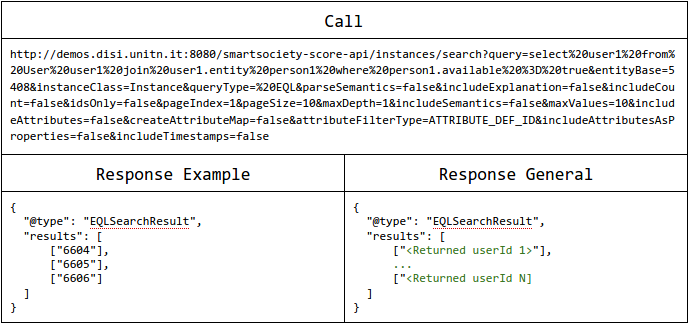
\includegraphics[width=1\linewidth]{figures/Peer-search.png}
\caption{Call and response for searching all available peers for a generic task. This call is used by WP6 (Orchestration) to obtain a list of users (that represent peers) that matches their set requirement.}
\label{fig:Peer-search}
\end{figure*}

\begin{figure*}[htb!]
\centering
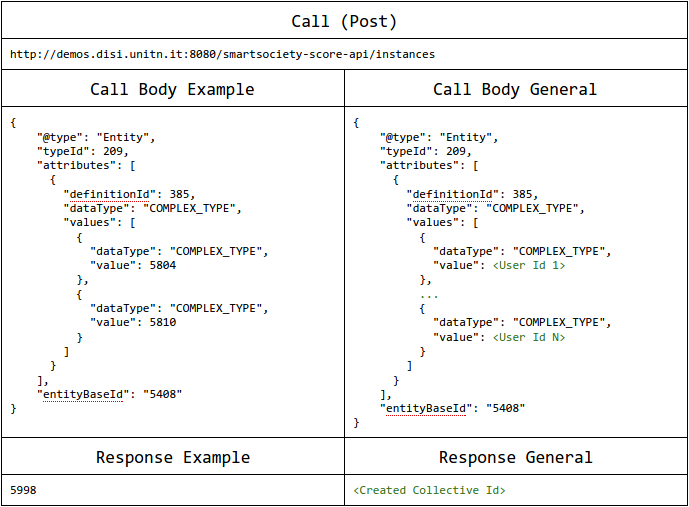
\includegraphics[width=1\linewidth]{figures/Collective-create.png}
\caption{Call and response for creating a new collective from a set of passed users. This call is used by the WP8 developed client to convert the list of users given by WP6 into a single Collective.}
\label{fig:Collective-create}
\end{figure*}

\begin{figure*}[htb!]
\centering
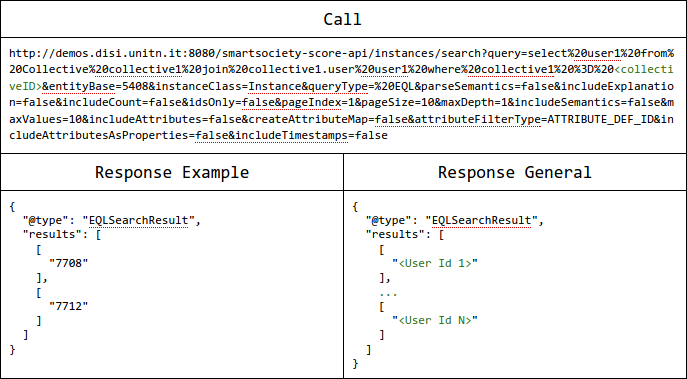
\includegraphics[width=1\linewidth]{figures/Collective-read.png}
\caption{Call and response for reading all the users from a given collective. WP7 (Middleware) uses this call to get the individual Users from a Collective with the intention of later contacting them.}
\label{fig:Collective-read}
\end{figure*}

\begin{figure*}[htb!]
\centering
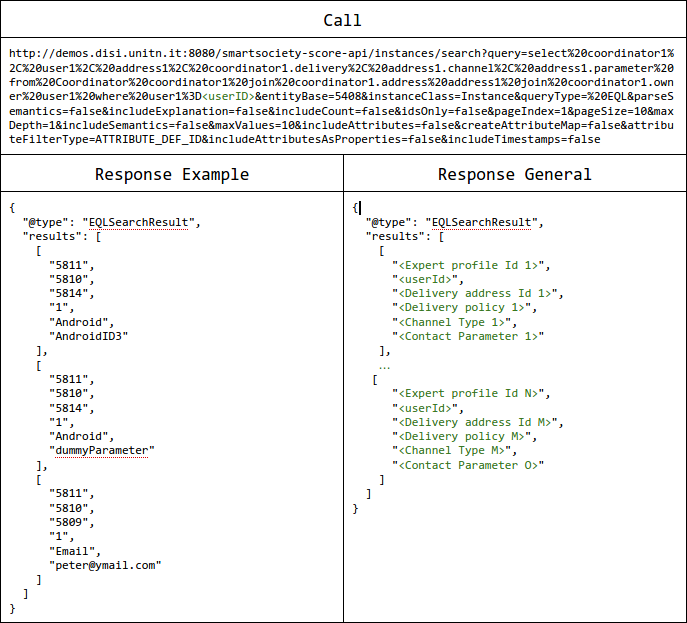
\includegraphics[width=1\linewidth]{figures/Peer-read.png}
\caption{Call and response for reading the contact information of a given peer. WP7 uses this call to get the specific contact preferences of a user in order to follow them when contacting that user.}
\label{fig:Peer-read}
\end{figure*}